\subsection{{\bf Comparison on Type Prediction (RQ2)}}
\label{empirical-rq2}



%{\color{red}{I found that the hityper and type4py have results on the dataset ManyTypes4PY. Our results are a little bit different from theirs. I think the reason is that we only use 25k+ while they use the full dataset. To make it consistent, I changed the numbers here in the table to the results that they got on the full dataset. But I still keep our results on google slides in case we need them.}}

While we focus on variable name prediction, the result of variable
type prediction is also important and useful because the types in the
minified code are exactly the same for the original code.  In this
study, we evaluate {\tool}'s accuracy and compare it with the
state-of-the-art approaches in variable type prediction. As seen in
Figure~\ref{type-prediction-result}, for all variables, {\tool}
achieves high top-1 accuracy of {\bf 79\%} for exact-matches of the
types and {\bf 89\%} for the parametric matches. That is, in 79\% of
the cases, it can recover the correct variable types with a single
prediction.
%For 89\% of the cases, the output type is correct without
%comparing the parameters' types.
%
The relative improvements in top-1 accuracy in exact-matching over
Ivanov {\em et al.}~\cite{ivanov21predicting}, TypeWriter\cite{typewriter-fse20},
Typilus~\cite{typilus-pldi20}, 
Type4Py~\cite{Type4Py-icse22}, and HiTyper~\cite{HiTyper-icse22} are
{\bf 51.9\%, 43.6\%}, {\bf 33.8\%}, {\bf 27.4\%}, and {\bf
  14.5\%}, respectively. The absolute improvements in top-1 accuracy
over those state-of-the-art type prediction approaches are from
10\%--27\%.

\begin{figure}[t]%[thbp]
\begin{center}
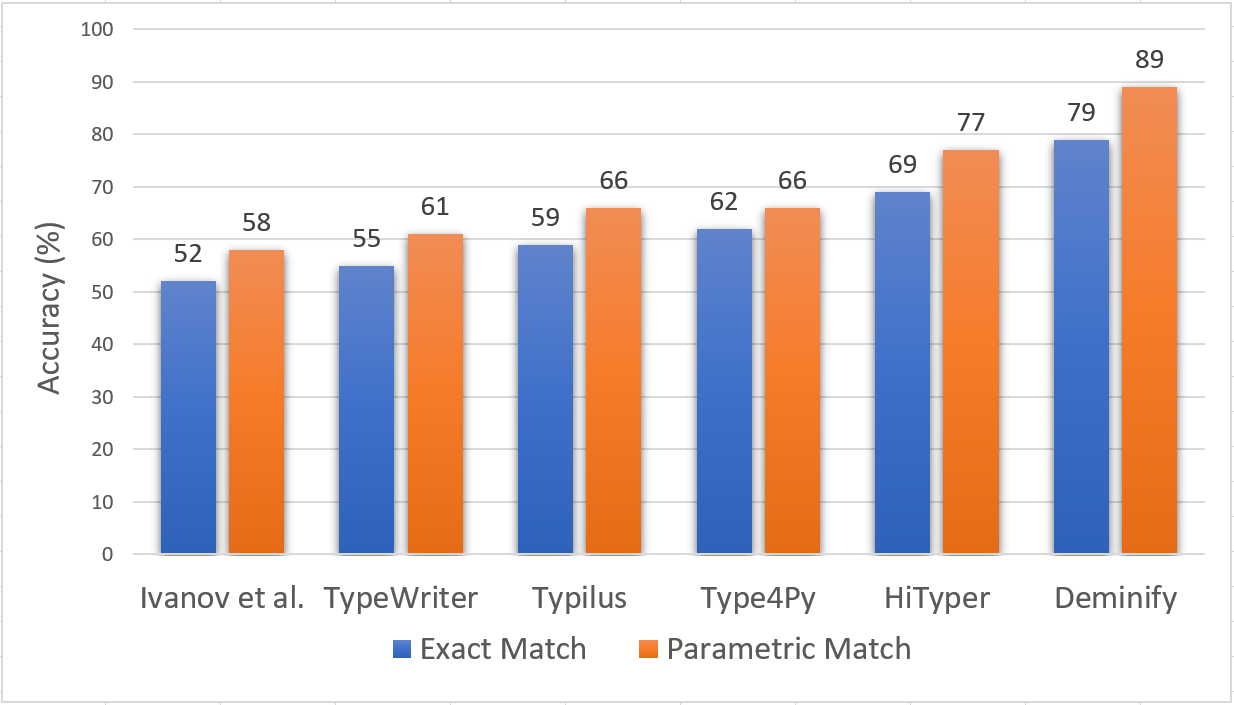
\includegraphics[width=3.1in]{figures/type-prediction-result-2}
\vspace{-8pt}
\caption{RQ2. Top-1 Accuracy on Type Prediction}
\label{type-prediction-result}
\end{center}
\end{figure}

Regarding the parametric matches (disregarding the types of the
parameters), {\tool} achieves higher top-1 accuracy. In 89\% of the
cases, it can recover the correct variable types (discarding those of
parameters) with a single prediction. The relative improvements in
top-1 accuracy in parametric-matching over Ivanov {\em et
  al.}~\cite{ivanov21predicting}, TypeWriter\cite{typewriter-fse20},
Typilus~\cite{typilus-pldi20}, Type4Py~\cite{Type4Py-icse22}, and
HiTyper~\cite{HiTyper-icse22} are {\bf 53.4\%, 45.9\%}, {\bf 34.8\%},
{\bf 34.8\%}, and {\bf 15.5\%}, respectively. The absolute
improvements in top-1 accuracy with parametric matching over the
state-of-the-art approaches are from 12\%--31\%.



Moreover, {\tool} also achieves high top-$k$ ($k$=3,5) accuracies: as
seen in Table~\ref{type-result}, in 88\% of the variables, the correct
types of the variables are in the list of five candidate types. The
relative improvements in top-5 accuracy in parametric-matching over
Ivanov {\em et al.}~\cite{ivanov21predicting}, TypeWriter\cite{typewriter-fse20},
Typilus~\cite{typilus-pldi20}, 
Type4Py~\cite{Type4Py-icse22}, and HiTyper~\cite{HiTyper-icse22} are
{\bf 46.6\%, 42\%}, {\bf 37.5\%}, {\bf 31.3\%}, and {\bf 22.2\%},
respectively.

%1. {\tool} performs the best comparing with all baselines by increasing the top-1, top-3, and top-5 accuracy by XX\%, XX\%, and XX\%

We examined the cases that {\tool} predicted correctly and the
baselines missed. Compared with HiTyper~\cite{HiTyper-icse22}, HiTyper
did not perform well for the isolated groups of a couple
variables. That is, the groups are isolated, i.e., not type-dependent
to other variables and HiTyper did not correctly detect any of those
variable types. In those cases, {\tool} could rely on the concordance
between the names and types of a variable. For example, the type of a
variable named \code{index} or \code{count} will likely be \code{int}.

Type4Py~\cite{Type4Py-icse22} uses a hierarchical neural network model
to learn to distinguish between similar/dissimilar types in a vector
space. The candidate types are predicted via nearest neighbor search.
In contrast, {\tool} also encodes the information on variable names
into the embeddings in the high-dimensional space via two mechanisms:
dual-task learning and cross-product of vectors. Thus, {\tool} could
perform better in the cases in which the embeddings for types are not
sufficiently distinguishable from one another, leading to low accuracy
for Type4Py. Regarding the used neural networks, it uses Recurrent
Neural Network (RNN) operating on the code token embeddings built from
the Abstract Syntax Tree (AST). In contrast, we use GCNmf that could
capture better the dependencies with different types of edges.

\begin{table}[t]%[htbp]
  \caption{RQ2. Comparison on Type Prediction}
  \vspace{-7pt}
	\begin{center}
		\small
		\renewcommand{\arraystretch}{1} \begin{tabular}{|p{1.9cm}<{\centering}|p{0.65cm}<{\centering}|p{0.65cm}<{\centering}|p{0.65cm}<{\centering}|p{0.65cm}<{\centering}|p{0.65cm}<{\centering}|p{0.65cm}<{\centering}|}
			
			\hline
                       & \multicolumn{2}{c|}{Top-1}         & \multicolumn{2}{c|}{Top-3}         & \multicolumn{2}{c|}{Top-5} \\
			\hline
                       & EM & PM & EM & PM & EM & PM  \\ 
			\hline
		        Ivanov {\em et al.}~\cite{ivanov21predicting} &  52    & 58     &   55   &  63     &  60     &   67    \\
			TypeWriter~\cite{typewriter-fse20}  &   55   &  61    &  59    &   66   &  62    &  70     \\
			Typilus~\cite{typilus-pldi20}  &   59   &  66    &  63    &  71    &  64    & 73      \\
                       	Type4Py~\cite{Type4Py-icse22}  & 62 & 66 & 66 & 72 & 67 & 73 \\
                        HiTyper~\cite{HiTyper-icse22}  & 69 & 77 & 72 & 81 & 72 & 82 \\
			\hline
			{\bf {\tool}}                        & 79 & 89 & 87 & 90 & 88 & 94 \\
			\hline
		\end{tabular}
		\label{type-result}
		{\bf EM}: Exact Match, {\bf PM}: Parametric Match
	\end{center}
\end{table}

Compared to Typilus~\cite{typilus-pldi20}, {\tool} relatively improves
31.6\% in top-1 accuracy. Similar to Type4Py, Typilus builds a vector
space for type embeddings. It uses a graph neural network to learn to
map variables, parameters, and function returns to a type embedding
space using deep similarity learning. For type inference, using the
type map, it accepts unannotated code, computes type embeddings with
the trained GNN and finds the concrete $k$ nearest neighboring types
as the candidates. There are two key limitations in Typilus that
{\tool} overcomes. First, their graph representation does not directly
encode the type dependencies. It encodes among the code tokens the
next-lexical-token relation, structural/syntactical relations, and
data dependencies. Second, it does not have the assistance of the
learning of variable names as the above explanation in the comparative
analysis with HiTyper.

TypeWriter~\cite{typewriter-fse20} extracts code tokens to build token
embeddings and uses two RNNs for identifiers and for code to merge
them to form type vectors. It then uses feedback-directed search on
the results from a static type checker to search for consistent types.
The key limitation is that the type dependencies are not encoded
during the learning. Instead, TypeWriter leverages an external static
type checker and relies on the feedback-directed searching for the
right types. If the RNN models do not produce the right types at the
first place, then the searching via a static type checker will not
result in any better output.

For Ivanov {\em et al.}~\cite{ivanov21predicting}, {\tool} has
the same advantages as the comparison to the above approaches
with graph embeddings.

%2. HiTyper is mainly based on the rules from python to predict the
%types. {\tool} performs similarly (and even slightly better) than
%HiTyper. It proves that {\tool} can work well on type prediction with
%less human effort on rules summarization. Also, {\tool} can easier be
%used on programming languages compared with HiTyper

%3. Type4py uses a hierarchical neural network with RNN layers to predict types. {\tool} could improve XX\% compared with Type4py because {\tool} learns both the variable representation vectors and different types of the variable relationships from the combined graphs while type4py relies on AST-structure that can show the relationship but cannot differ the different types of relationships.

%4. Typilus uses a graph model to learn the relationship to predict variable types. {\tool} could improve XX\% compared with Typilus because {\tool} uses dual learning, and the name prediction results can help improve the accuracy of the type prediction.

%5. Ivanov et al.\cite{ivanov21predicting} uses simple CNN models to predict variable types. {\tool} could improve XX\% compared with Ivanov et al.\cite{ivanov21predicting} because {\tool} uses a combined graph with the graph-based model to predict types, and the combined graph can represent the variable relationship better than the sequential order of tokens. These relationships can help predict the types with higher accuracy.

%6. TypeWriter is similar to Type4py, and it is also based on AST structure. For the similar reason explained in point 3, {\tool} can outperform TypeWriter by XX\%.
